% -*- mode: fundamental -*-

% ****************************************************************

\chapter{Struct types {\large (BSV)}\\
Memory requests and responses {\large (RISC-V)}}

\markboth{Ch \arabic{chapter}: Structs, mem reqs and rsps (DRAFT)}{\copyrightnotice}

\setcounter{page}{1}
% \renewcommand{\thepage}{\arabic{page}}
\renewcommand{\thepage}{\arabic{chapter}-\arabic{page}}

\label{ch_Structs_Mem_Reqs_Rsps}

% ****************************************************************

\section{RISC-V: structs communicated between steps}

\index{BSV!struct!hetoregeneous collection of values}
\index{BSV!field!of a {\tt struct}}
\index{BSV!member!of a {\tt struct}}


Various kinds of information need to be communicated between the steps
of Figure~\ref{Fig_Instr_Exec}---program counter values, instructions,
values read from registers, values to be written back to registers,
and so on.  \verb|struct| data types (short for ``structures'') are
suitable for bundling together heterogeneous collections of values.
(This is the same concept in C and SystemVerilog; it is also called a
``record'' in some programming languages.)  Each component of a struct
is called a ``field'' or a ``member'' of the struct.

\begin{figure}[htbp]
  \centerline{\includegraphics[width=6in,angle=0]
             {ch030_RISCV_Design_Space/Figures/Fig_Instr_Exec_w_structs}}
  \caption{\label{Fig_Simple_Instr_Exec_w_structs}
           Simple interpretation of RISC-V instructions
	   (Fig.~\ref{Fig_Instr_Exec} with arrows annotated with {\tt struct} types)}
\end{figure}
Figure~\ref{Fig_Simple_Instr_Exec_w_structs} annotates
Figure~\ref{Fig_Instr_Exec} with struct types communicated on each of
the black arrows between steps, and each of the red arrows to and from
memory.  In this and the next few chapters we will flesh out the
details of all these struct types.  We will use exactly the same
struct types for Fife and Drum, {\ie} whether the implementation is
pipelined or not.

% ****************************************************************

\section{BSV: {\tt struct} types}

\label{BSV_struct_types}

Consider the black arrow from the Decode step to the
Register-read-and-Dispatch step of
Figure~\ref{Fig_Simple_Instr_Exec_w_structs}.
We want to communicate several values, including:

\begin{itemize}

\item The current PC.  This will be needed by BRANCH, JAL, JALR and
  AUIPC instructions to compute addresses that are offset from the
  current PC.  It will be needed for any traps (exceptions) that may
  occur, which save PC for the trap-handler.

\item An \verb|exception| flag, indicating:

  \begin{tightlist}

    \item whether an error was encountered in the Fetch-to-Memory-to-Decode path, or

    \item whether the Decode step's analysis indicates that the
        instruction is not legal (unrecognized 32-bit code).

  \end{tightlist}

  When the exception flag is true, a \verb|cause| field provides more detail.

\item If there is no exception (no Fetch memory error; instruction is
legal), other fields provide more analytical detail for subsequent steps:

  \begin{tightlist}

    \item The ``fall-through'' PC, {\ie} the address of the next
      instruction following this one in memory.  For RV32I and RV64I,
      this will always be PC+4, since all instructions are 4-bytes
      long.\footnote{If we implement the ``C'' RISC-V ISA extension
      (compressed instructions), the correct fall-through PC may be
      PC+2.}  For most instructions, the fall-through PC is indeed the
      unique next PC.  For conditional BRANCH instructions, this is
      the next PC if the BRANCH is not taken.  For JAL and JALR
      instructions (unconditional jumps), this is the ``return
      address'' saved by the instruction in a register.

    \item The instruction itself.  This will be needed for opcode
      details, the rs1, rs2 and rd register indexes, immediate values,
      {\etc}
  \end{tightlist}

  The next several fields are derived by analyzing the instruction.
  They could be re-derived wherever needed by re-analyzing the
  instruction, but we perform that work just once in the Decode step
  and communicate the results.

  \begin{tightlist}

    \item The \verb|OpClass|.  This indicates to which next-step in
      Figure~\ref{Fig_Simple_Instr_Exec_w_structs} we dispatch for
      subsequent actions.

    \item Whether the instruction reads rs1 and/or rs2 register
      values.  This will be needed to control reading from the
      register file.

    \item Whether the instruction writes an rd register value.  This
      will be needed to control writing to the register file.

    \item The ``immediate'' value in the instruction. Refer to the top
        of each page of ``Table 24.2 Instruction listing for RISC-V''
        in the Unprivileged Spec~\cite{RISCV_Unpriv_2019_12_13}, which
        shows that the I-, S-, B-, U- and J-type instructions have
        immediate values of different sizes and encode them in
        different ways (``bit-swizzled'').  We untangle these once in
        the Decode stage, and pass on the clarified results in the
        \verb|imm| field.
  \end{tightlist}

\end{itemize}

This heterogeneous collection of values is most conveniently expressed
as a \verb|struct| type:

\index{BSV!struct@{\tt struct}!type declaration}

\begin{Verbatim}[frame=single, numbers=left]
typedef struct {Bit #(XLEN)  pc;

		Bool         exception;
		Bit #(XLEN)  cause;      // Memory exception during Fetch;
                                         // Illegal instr decoded.
		// If not exception
		Bit #(XLEN)  fallthru_pc;
		Bit #(32)    instr;
                OpClass      opclass;
		Bool         has_rs1;
		Bool         has_rs2;
		Bool         has_rd;
		Bit #(32)    imm;          // Canonical (bit-swizzled)
} D_to_RR
deriving (Bits, FShow);
\end{Verbatim}

% ----------------

\index{BSV!deriving!Bits}

Because we said ``\verb|deriving(Bits)|'', the \emph{bsc} compiler
will automatically work out a representation for \verb|D_to_RR| values
in bits, using the straightforward method of simply concatenating the
bit-vectors of each field into a bit-vector for the whole struct.  The
total bit-size of a \verb|D_to_RR| struct value is simply the sum of
the individual bit-sizes of the fields.  If we had not said
``\verb|deriving(Bits)|'', we could explicitly provide some other
custom representation in bits.\footnote{ In C/C++, compilers will
often ``pad'' out fields (insert unused bits between fields) to be
aligned on byte and word boundaries, for more efficient access in
byte-structured memories; thus, a struct's size in C/C++ may be larger
than the sum of the field sizes, and may even vary depending on the
compiler's target architecture.  In hardware design, these values may
reside in wires, registers, FIFOs, etc which have no
``byte-structured'' bias, and so we do not play any such ``padding''
games.}

% ----------------

\index{BSV!deriving!Fshow}

Because we said ``\verb|deriving(FShow)|'', the \emph{bsc} compiler
will automatically define an ``\verb|fshow()|'' function for this
type: if we print \verb|fshow(|\emph{v}\verb|)|, it will print
something like this:

\begin{quote}\tt
D\_to\_RR \{inum=..., pc=..., instr=..., ... \}
\end{quote}

% ================================================================

\subsection{Creating struct values}

\index{BSV!struct!entire struct values}

We can create a new value of type \verb|D_to_RR| with syntax like
this:

\begin{Verbatim}[frame=single, numbers=left]
      D_to_RR x = D_to_RR {pc:           ... value of field ... ,
                           exception:    ... value of field ... ,
                           cause:        ... value of field ... ,
                           fallthru_pc:  ... value of field ... ,
                           instr:        ... value of field ... ,
                           ...};
\end{Verbatim}

The right-hand side is sometimes called a ``struct expression'', {\ie}
it is an expression which, when evaluated, produces a struct value.

The repetition of \verb|D_to_RR| above seems verbose; the left-hand
side instance is the type, and the right-hand side instance is the
``struct constructor'' (think of it as a function that takes the field
values as arguments and returns a struct value). The \emph{bsc}
compiler's type-analysis is able to infer the type from the right-hand
side, so we can just use the keyword ``\verb|let|'':

\index{BSV!let@{\tt let}!binding an identifier with implicit type declaration}
\index{let@{\tt let}!BSV: binding an identifier with implicit type declaration}

\begin{Verbatim}[frame=single, numbers=left]
      let x = D_to_RR {pc:           ... value of field ... ,
                       exception:    ... value of field ... ,
                       cause:        ... value of field ... ,
                       fallthru_pc:  ... value of field ... ,
                       instr:        ... value of field ... ,
                       ...};
\end{Verbatim}

The order in which the field values are given does not matter; the
\emph{bsc} compiler will put the fields into the correct offsets in
the struct value.

Not all field values need be given in a struct expression.  The
\emph{bsc} compiler will issue a warning for each unspecified field,
and insert an ``unspecified'' (and unpredictable) values.  You can
indicate that a field is intentionally left unspecified (and suppress
the compiler warning) using a ``\verb|?|'':

\begin{Verbatim}[frame=single, numbers=left]
      let x = D_to_RR {pc:           ... ,
                       exception:    False,
                       cause:        ?,
                       fallthru_pc:  ... ,
                       instr:        ... ,
                       ...};
\end{Verbatim}

In the above example, the exception \verb|cause| field is meaningless
when the \verb|exception| field is false, and we indicate explicitly
this with ``\verb|?|''.\footnote{ In the RTL languages Verilog,
SystemVerilog and VHDL, there is a concept of ``X'' (unassigned)
values. In BSV there is no such concept; thus ``{\tt ?}'' repesents
some legitimate--but unspecified--binary value.  Note that even in the
RTL languages, ``X'' has meaning only in simulators, not in real
hardware, where it also becomes some legitimate--but
unspecified--binary value.}

% ================================================================

\subsection{Selecting struct fields}

\index{BSV!struct!field selection}

Struct fields can be selected using the usual ``dot'' notation common
to SystemVerilog and C/C++:

\begin{Verbatim}[frame=single, numbers=left]
x.pc
x.instr
\end{Verbatim}


% ================================================================

\subsection{Updating struct fields using assignment}

\index{BSV!struct!field assignment/update}

Struct fields can be updated with assignment using the usual ``dot''
notation common to SystemVerilog and C/C++:

\begin{Verbatim}[frame=single, numbers=left]
x.pc    = ... new value ... ;
x.instr = ... new value ... ;
\end{Verbatim}

% ****************************************************************

\section{RISC-V: Memory Requests and Responses; IMem and DMem}

\index{IMem| Instruction Memory}
\index{DMem| Data Memory}
\index{RISC-V!IMem (instruction memory)}
\index{RISC-V!DMem (data memory)}

In Figure~\ref{Fig_Simple_Instr_Exec_w_structs}, the \verb|Mem_Req|
and \verb|Mem_Rsp| structs are used in two places.  The Fetch step
issues a memory request, and the corresponding memory response is
received by the Decode step.  Similarly, the ``Execute Memory Ops''
steps issues a memory request and consumes a memory response.  We use
the shorthand term ``IMem'' for the first context (for Instruction
Memory) and ``DMem'' for the latter context (for Data Memory).

% ================================================================

\subsection{Separation of IMem and DMem (Harvard Architecture)}

\index{Harvard architecture}
\index{Harvard architecture!Self-modifying code}

The separation of memory channels for instructions and data
(loads/stores) is quite standard in modern CPU architectures, and is
informally called a ``Harvard Architecture''.  The term refers to the
architecture of the Harvard Mark I computer, designed and built by
Harvard University and IBM in the 1940s (the term itself was coined
much later).  It sometimes refers just to separate, concurrent paths
to memory for instructions and data, and sometimes also to physically
separate memories for instructions and data (more discussion in
Wikipedia:~\url{https://en.wikipedia.org/wiki/Harvard_architecture}).

Modern software is typically not ``self-modifying'', {\ie}
instructions and data are placed in different areas of memory, and
load/store instructions never write into the instruction area, {\ie}
programs never over-write instructions in memory.  This allows
separate hardware for memory access for instructions {\vs} memory
access for data, which can run concurrently, {\ie} we may fetch an
instruction at the same time as we are accessing data memory for a
previous load/store instruction (we will see this in Fife).  We can
also tune and optimize each memory path separately for their different
dynamic behavioral patterns.  In some systems we can also
\emph{protect} the instruction memory area, {\ie} enforce in hardware
the policy of not over-writing instructions.

\index{JIT!Just-in-time compiling}
\index{Just-in-time compiling!JIT}

This view of strict separation of IMem and DMem has to be tempered
somewhat when considering languages like JavaScript, Python {\etc}
that employ so-called ``JIT'' compiling (``Just-In-Time'').  The
run-time systems of such languages generate instructions on-the-fly,
{\ie}, LOAD/STORE instructions produce \emph{data} through the DMem
channel that will (soon) be fetched as \emph{instructions}.  But even
in these systems, there is a strict protocol of \emph{phases}.  During
a code-generation phase, the data produced is considered as ordinary
data.  Then there is a deliberately executed phase-change, where the
virtual memory protections of the data-pages just written are changed
so that they are now viewed as read-only instruction pages, after
which these new instructions can be fetched.

% ================================================================

\subsection{RISC-V: Memory Requests}

\index{Memory!Request}

A memory-request is either for reading data (``LOAD'') or for writing
data (``STORE'').\footnote{When implementing the ``A'' RISC-V ISA
extension (Atomic Ops), memory requests can also be for LR
(Load-Reserved), SC (Store-Conditional), AMOSWAP, AMOADD, AMOXOR,
AMOAND, AMOOR, AMOMIN, AMOMAX, AMOMINU, and AMOMAXU.}  We can express
these request-types using an enum type (similar to enums in C or
SystemVerilog):

\begin{Verbatim}[frame=single, numbers=left]
typedef enum {MEM_REQ_LOAD,
	      MEM_REQ_STORE} Mem_Req_Type
deriving (Eq, FShow, Bits);
\end{Verbatim}

An IMem request is for one 32-bit instruction (four
bytes).\footnote{When implmenting the ``C'' RISC-V ISA extension
(compressed instructions), instructions can also be 16-bits (2 bytes).
When implementing more sophisticated Fetch units, we may actually
fetch much larger chunks, such as a full cache line.}  A DMem request
may be for one, two or four bytes.\footnote{In RV64, and with the
``D'' RISC-V ISA extension for double-precision floating-point even in
RV32, memory-requests can also be for eight bytes.}  We express these
request-size options using an enum type:

\begin{Verbatim}[frame=single, numbers=left]
typedef enum {MEM_1B, MEM_2B, MEM_4B} Mem_Req_Size
deriving (Eq, FShow, Bits);
\end{Verbatim}

A memory request bundles a request type, a size, and an address.  For
memory-writes, we also bundle the data to be stored.  We express this
bundle using a struct:

\begin{Verbatim}[frame=single, numbers=left]
typedef struct {Mem_Req_Type  req_type;
		Mem_Req_Size  size;
		Bit #(XLEN)   addr;
		Bit #(XLEN)   data;    // Only for STORE
} Mem_Req
deriving (Eq, FShow, Bits);
\end{Verbatim}

For STORE requests of 1 and 2 bytes ({\ie} smaller than the \verb|data|
field) we assume the data is passed in the least-significant bytes of
the \verb|data| field.

This is the information sent to Memory from the Read-PC-and-Fetch step
and also from the Execute-Memory-Ops step in
Figure~\ref{Fig_Simple_Instr_Exec_w_structs}.

% ================================================================

\subsection{RISC-V: Address Alignment}

\index{Address alignment}
\index{Memory!Address alignment}

Although nowadays we think of all computer memories in units of 8-bit
bytes and being byte-addressed,\footnote{Some early computers, until
about the late 1970s, had other memory granularities---multiples of 6,
7, 9 bits, {\etc} Those were the days of bespoke memories for each
computer design.  Mass-production of memory chips resulted in
standardization to 8-bit bytes.} in practice in hardware, it is
usually simpler if memory-requests are \emph{aligned} to an address
according to the request size.  Specifically, the address for a 2-byte
request should be even, {\ie} the least significant bit of the
address, \verb|addr[0]|, should be zero.  The address for a 4-byte
request should have zero in the two least significant bits
(\verb|addr[1:0]|) and the address for an 8-byte request should have
zero in the three least significant bits (\verb|addr[2:0]|).

We can see why address-alignment is desirable.  Memory implementations
(chips) are usually architected to retrieve multiple bytes at a time
({\eg} 64 bytes) so that all those bytes can share addressing and
control circuitry.  With such an organization, a misaligned access
request may straddle the boundaries of such ``naturally sized'' units
and so may require two consecutive reads/writes.  Caches are usually
organized to hold multi-byte \emph{cache lines} ({\eg}, 32 bytes) in
order to share the addressing and miss-handling circuitry, and to move
data efficiently in and out of the cache.  Again, a misaligned access
request may straddle a cache-line boundary, and may require two
consecutive accesses, which may hit or miss independently.  Virtual
memory systems are usually organized in \emph{pages}, units of
typically 4K-8K bytes, in order to share virtual-memory handling
circuitry, and to move data efficiently between main memory and disks.
Again, a misaligned access may straddle a page boundary, and may
require two consecutive accesses, which may hit or page-fault
independently and differently.  In short, misaligned accesses add
significant complexity to memory-system hardware design.

We can organize our software so that misaligned accesses are
exceedingly rare.  Most software is produced by compilers, and the
compiler ensures that instructions and data are placed in memory at
aligned addresses, possibly by padding gaps between ``adjacent''
smaller-sized data (such as a pair of 1-byte-sized fields in a
struct).  This padding may waste a few bytes of memory, but pays back
in greater speed and reduced complexity.

Although misaligned accesses are rare, we cannot always guarantee
their absence in software, since software can calculate an arbitrary
address before performing a memory access.  It seems wasteful to have
to pay for extra hardware complexity (with attendant loss in overall
performance) for such rare cases.  In many computer systems,
therefore, these rare misaligned accesses are relegated to software
handling:

\begin{tightlist}

\item The memory system simply refuses to handle a misaligned access,
  and returns a ``misaligned'' error instead.

\item The CPU, receiving such an error response, undergoes a ``trap''
  which directs it to piece of software called an trap-handler (or
  exception handler).  The trap-handler (in software) performs the
  memory access in multiple smaller pieces (in the worst case, of size
  1 byte), each of which is aligned.  In other words, the trap-handler
  ``completes'' the original memory access before resuming the
  main-line code that attempted it.

\end{tightlist}

The RISC-V ISA specification does not forbid misaligned accesses nor
prescribe how they should be handled.  Some implementations will
handle it in hardware, and other implementations will return a
``misaligned'' error and rely on a trap handler to complete the
access.  Some implementations may only run software where it has been
proven to not generate misaligned memory requests, and therefore may
not even contain a trap-handler for misaligned accesses.

% ================================================================

\subsection{RISC-V: Memory Responses}

\index{Memory!Response}

The response from memory for any request may be to report success, an
alignment error, or some other error.  Examples of ``other errors''
are:

\begin{itemize}

\item Absence of memory at the given address.  For example, although
  RV32I addresses are 32-bits, which can address 4GiB of memory, we
  may provision our system with something smaller, say 1 GiB.

\item An unsupported operation. {\Eg} an attempt to write into a
  read-only memory (ROM).

\item Corruption of data, due to electrical glitches, environmental
  electromagnetic pulses, {\etc}.  These errors are usually detected
  with some kind of error-detecting code, such as parity bits.

\end{itemize}

These different memory response-types can be encoded in an enum type:

\begin{Verbatim}[frame=single, numbers=left]
typedef enum {MEM_RSP_OK,
              MEM_RSP_MISALIGNED,
	      MEM_RSP_ERR         } Mem_Rsp_Type
deriving (Eq, FShow, Bits);
\end{Verbatim}

A memory-response contains the response-type and, for a LOAD request
with an OK, the data that was read from memory.  This can be expressed
in a struct:

\begin{Verbatim}[frame=single, numbers=left]
typedef struct {Mem_Rsp_Type  rsp_type;
		Bit #(XLEN)   data;    // Only for LOAD
} Mem_Rsp
deriving (Eq, FShow, Bits);
\end{Verbatim}

For LOAD requests of 1 and 2 bytes ({\ie} smaller than the \verb|data|
field) we assume the data is returned in the least-significant bytes
of the \verb|data| field.

% ****************************************************************

\section{RISC-V: The Decode function}

\label{Sec_Combo_Decode}

\index{Drum!Decode function}

We are now in a position to write \verb|fn_D|, the Decode function in
Figure~\ref{Fig_Simple_Instr_Exec_w_structs}:

\begin{Verbatim}[frame=single, numbers=left]
function D_to_RR
         fn_D (F_to_D x_F_to_D, Mem_Rsp rsp_IMem);

   Bit #(32) instr = truncate (rsp_IMem.data);
   Bit #(5)  rd    = instr_rd (instr);

   let fallthru_pc = x_F_to_D.pc + 4;

   // Baseline info to next stage
   let y = D_to_RR {pc:           x_F_to_D.pc,

                    exception:    False,
                    cause:        ?,

                    // not-exception
                    fallthru_pc: fallthru_pc,
                    instr:       instr,
                    opclass:     ?,
                    has_rs1:     False,
                    has_rs2:     False,
                    has_rd:      False,
                    writes_mem:  False,
                    imm:         0};

   if (rsp_IMem.rsp_type == MEM_RSP_MISALIGNED) begin
      y.exception = True;
      y.cause     = cause_INSTRUCTION_ADDRESS_MISALIGNED;
   end
   else if (rsp_IMem.rsp_type == MEM_RSP_ERR) begin
      y.exception = True;
      y.cause     = cause_INSTRUCTION_ACCESS_FAULT;
   end
   else if (is_legal_LUI (instr) || is_legal_AUIPC (instr)) begin
      y.opclass = OPCLASS_IALU;
      y.has_rd  = non_zero_rd;
      y.imm     = zeroExtend (instr_imm_U (instr));
   end
   else if (is_legal_BRANCH (instr)) begin
      y.opclass = OPCLASS_CONTROL;
      y.has_rs1 = True;
      y.has_rs2 = True;
      y.imm     = zeroExtend (instr_imm_B (instr));
   end
   else if (is_legal_JAL (instr)) begin
      y.opclass = OPCLASS_CONTROL;
      y.has_rd  = non_zero_rd;
      y.imm     = zeroExtend (instr_imm_J (instr));
   end
   else if (is_legal_JALR (instr)) begin
      y.opclass = OPCLASS_CONTROL;
      y.has_rs1 = True;
      y.has_rd  = non_zero_rd;
      y.imm     = zeroExtend (instr_imm_I (instr));
   end
   else if (is_legal_LOAD (instr)) begin
      y.opclass = OPCLASS_MEM;
      y.has_rs1 = True;
      y.has_rd  = non_zero_rd;
      y.imm     = zeroExtend (instr_imm_I (instr));
   end
   else if (is_legal_STORE (instr)) begin
      y.opclass    = OPCLASS_MEM;
      y.has_rs1    = True;
      y.has_rs2    = True;
      y.writes_mem = True;
      y.imm        = zeroExtend (instr_imm_S (instr));
   end
   else if (is_legal_OP_IMM (instr)) begin
      y.opclass = OPCLASS_IALU;
      y.has_rs1 = True;
      y.has_rd  = non_zero_rd;
      y.imm     = zeroExtend (instr_imm_I (instr));
   end
   else if (is_legal_OP (instr)) begin
      y.opclass = OPCLASS_IALU;
      y.has_rs1 = True;
      y.has_rs2 = True;
      y.has_rd  = non_zero_rd;
   end
   else if (is_legal_ECALL (instr) || is_legal_EBREAK (instr)) begin
      y.opclass = OPCLASS_SYSTEM;
   end
   else if (is_legal_FENCE (instr) || is_legal_FENCE_I (instr)) begin
      y.opclass = OPCLASS_FENCE;
      y.has_rs1 = True;
      y.has_rd  = non_zero_rd;
   end
   else begin
      y.exception = True;
      y.cause     = cause_ILLEGAL_INSTRUCTION;
   end

   return y;
endfunction
\end{Verbatim}

Note the use of functions \verb|instr_imm_I()|, \verb|instr_imm_S()|,
\verb|instr_imm_B()|, \verb|instr_imm_U()| and \verb|instr_imm_J()|,
which extract the ``immediate'' field from a 32-bit instruction.  For
the different classes of instruction (I, S, B, U, J), the immediates
are coded differently, and have different widths.  These functions
decode the bits and zero-extend them to XLEN bits (the width of
\verb|d_to_rr.imm|).  Later, in the ``execute'' code for each
instruction, we will pick out the relevant bits out of the XLEN bits,
and zero-extend or sign-extend them as needed for the particular
instruction.

An exercise below suggests that you write the code for these
\verb|instr_imm_X| functions.

Observe that the entire \verb|fn_D()| function is just a (large)
combinational circuit---it is an acyclic composition of smaller
combinational circuits, many of which we've seen earlier.

% ================================================================

\hdivider

% ----------------
\Exercise

Write the functions \verb|instr_imm_I()|, \verb|instr_imm_S()|,
\verb|instr_imm_B()|, \verb|instr_imm_U()| and \verb|instr_imm_J()|.

% ----------------
\Exercise

Write a testbench for \verb|fn_D()|, apply it on a number of 32-bit
values (instructions) and print the results.

\Endexercise

% ****************************************************************
